\section{Définitions}
\begin{defi}%Fonctions récusives]
Une fonction récursive est une fonction qui s'appelle elle-même.

On appelle récursion l'appel de la fonction à elle-même.
\end{defi}

La programmation récursive est un paradigme de programmation au même titre que la programmation itérative. Un programme écrit de manière récursive peut être traduit de manière itérative, même si dans certains cas, cela peut s'avérer délicat.


\begin{methode}
\begin{itemize}
\item Une fonction récursive doit posséder une condition d'arrêt (ou cas de base).
\item Une fonction récursive doit s'appeler elle-même (récursion).
\item L'argument de l'étape de récursion doit évoluer de manière à se ramener à la condition d'arrêt.
\end{itemize}
\end{methode}
 
 



\section{Suites définies par récurrence}

Les suite définies par récurrence pour lesquelles $u_{n}=f\left(u_{n-1},u_{n-2},...\right)$ sont des cas d'application directs des fonctions récursives. 

Par exemple, soit la suite $u_n$ définie par récurrence pour tout $n\in\mathbb{N}^*$ par 
$
\left\{
\begin{array}{ll} 
u_1 = 1 \\
u_{n+1} = \dfrac{u_n + 6}{u_n + 2} \\
\end{array}
\right.
$. Il est possible de calculer le n\ieme \, terme par un algorithme itératif ou un algorithme récursif. 

\noindent\begin{minipage}[c]{.45\linewidth}
\begin{lstlisting}
def un_it (n : int) -> float :
    if n == 1 :
        return 1
    else : 
        u = 1
        for i in range(2,n+1):
            u = (u+6)/(u+2)
        return u
\end{lstlisting}
\end{minipage} \hfill
\begin{minipage}[c]{.45\linewidth}
\begin{lstlisting}
def un_rec (n : int) -> float :
    if n == 1 :
        return 1
    else : 
        return (un_rec(n-1)+6)/(un_rec(n-1)+2)
\end{lstlisting}
\end{minipage} 

La figure suivante montre que dans le cas de l'algorithme récursif proposé plusieurs termes sont calculés à plusieurs reprises ce qui constitue une perte de temps et d'espace mémoire. 

\begin{center}
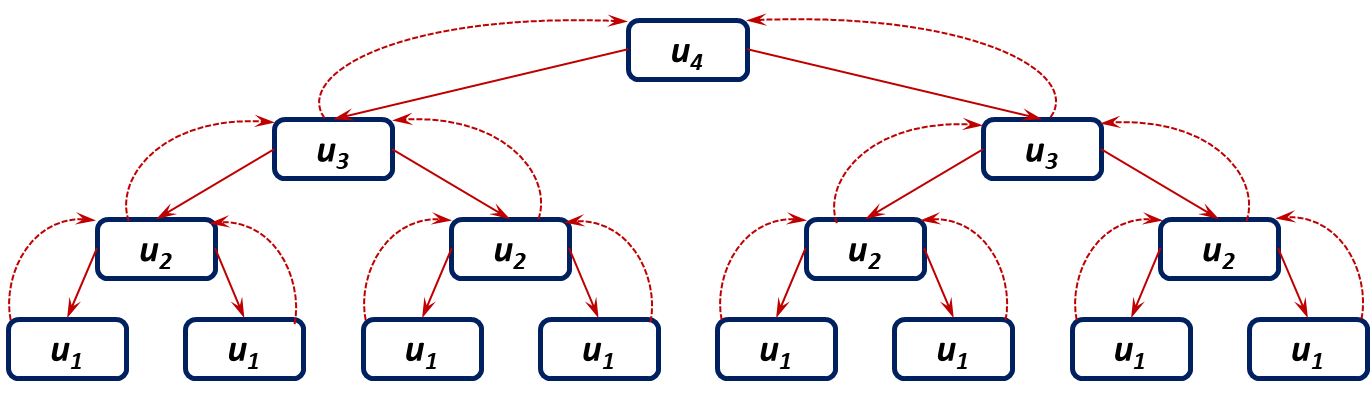
\includegraphics[width=.8\linewidth]{fig_01}
\end{center}

Une autre formulation de l'algorithme récursif permet très simplement de diminuer le nombre de termes calculés. 



\noindent\begin{minipage}[c]{.45\linewidth}
\begin{lstlisting}
def un_rec_v2 (n : int) -> float :
    if n == 1 :
        return 1
    else : 
        v = un_rec_v2(n-1)
        return (v+6)/(v+2)
\end{lstlisting}
\end{minipage} \hfill
\begin{minipage}[c]{.45\linewidth}
\begin{center}
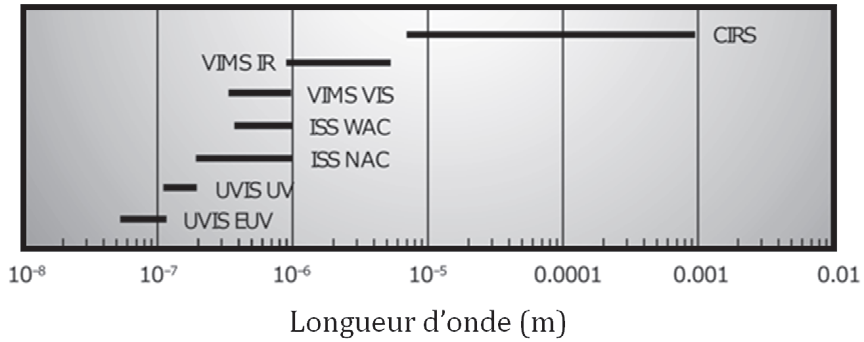
\includegraphics[width=.8\linewidth]{fig_02}
\end{center}\end{minipage}


Dans la même idée que les graphes présentés ci-dessus, il est possible de représenter la pile des appels récursifs, c'est à dire la succession des appels qui vont être faits pour calculer le nième terme d'une suite. 

\begin{center}
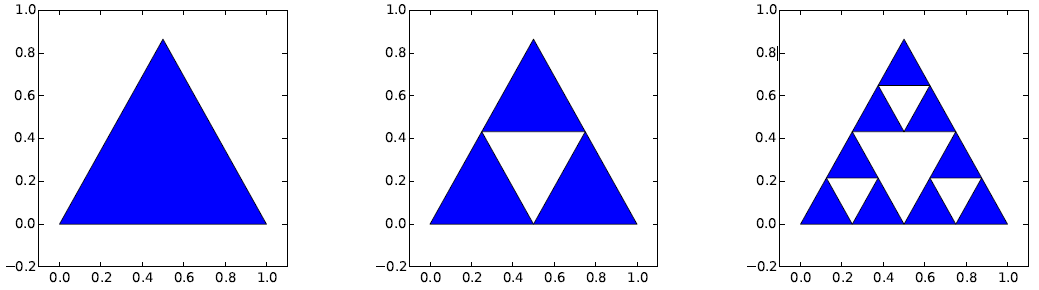
\includegraphics[width=.95\linewidth]{fig_04}
\end{center}

\section{Slicing de tableau ou de chaînes de caractères}
Il est possible d'agir par récursivité sur des listes ou sur des chaînes de caractère. Pour cela, il peut être nécessaire d'utiliser le slicing. Pour rappel, \texttt{a = ch[i:j]} permet d'affecter à \texttt{a} la liste (ou le chaîne de caractéres) constitué des éléments de \texttt{i} (inclus) à \texttt{j} (exclus). En écrivant \texttt{a = ch[i:]} on affecte à \texttt{a} tous les éléments du ième au dernier.


\vspace{.5cm}

\noindent\begin{minipage}[c]{.45\linewidth}

Ainsi, pour réaliser la somme des éléments d'une liste \texttt{L} par récusivité : 
\begin{itemize}
\item commençons par déterminer le cas terminal : si la taille de la liste vaut 1, on renvoie \texttt{L[0]};
\item sinon (si la taille vaut \texttt{n}), on peut choisir de renvoyer \texttt{L[0]}+\texttt{somme(L[1]+L[2]+...+L[n-1])}. 
\end{itemize}
Cela se traduit ainsi.
\begin{lstlisting}
def somme(L:list) -> float :
    if len(L)==1 : 
        return L[0]
    else :
        return L[0]+somme(L[1:])
\end{lstlisting}
\end{minipage} \hfill
\begin{minipage}[c]{.45\linewidth}
Pour une chaîne de caractères, si on souhaite renvoyer son miroir (par exemple, le miroir de \texttt{abc} serait \texttt{cba}) : 
\begin{itemize}
\item si la chaîne de caractère a une taille de 1, on renvoie le caractère;
\item sinon, on renvoie la concatanéation de  \texttt{miroir(ch[1:])+ch[0]}.
\end{itemize}
\begin{lstlisting}
def miroir(ch:str) -> str :
    if len(ch)==1 : 
        return ch[0]
    else :
        # Attention le + désigne la concaténation
        return miroir(ch[1:])+ch[0]
 \end{lstlisting}  
\end{minipage} 

\section{Algorithmes dichotomiques -- Diviser pour régner}

Les algorithmes dichotomiques se prêtent aussi à des formulations récursives. Prenons comme exemple la recherche d'un élément dans une liste triée. L'algorithme de gauche propose une version itérative. L'algorithme de droite une version récursive. 

\noindent\begin{minipage}[c]{.49\linewidth}
\begin{lstlisting}
def appartient_dicho(e : int , t : list) -> bool:
    """Renvoie un booléen indiquant si e est 
    dans t. Préconditions : t est un tableau 
    de nombres trié par ordre croissant e est 
    un nombre"""
    # Limite gauche de la tranche où l'on recherche e
    g = 0 
    # Limite droite de la tranche où l'on recherche e
    d = len(t)-1 
    # La tranche où l'on cherche e n'est pas vide
    while g <= d: 
        # Milieu de la tranche où l'on recherche e
        m = (g+d)//2 
        pivot = t[m]
        if e == pivot: # On a trouvé e
            return True
        elif e < pivot:
            # On recherche e dans la partie gauche de la tranche
            d = m-1 
        else:
            # On recherche e dans la partie droite de la tranche
            g = m+1 
    return False
\end{lstlisting}
\end{minipage} \hfill
\begin{minipage}[c]{.49\linewidth}
\begin{lstlisting}
def appartient_dicho_rec(e : int , t : list) -> bool:
    """Renvoie un booléen indiquant si e est dans t. Préconditions : t est un tableau de nombres trié par ordre croissant e est un nombre"""
    # Limite gauche de la tranche où l'on recherche e
    g = 0 
    # Limite droite de la tranche où l'on recherche e
    d = len(t)-1 
    # La tranche où l'on cherche e n'est pas vide
    while g <= d:
        # Milieu de la tranche où l'on recherche e 
        m = (g+d)//2 
        pivot = t[m]
        if e == pivot: # On a trouvé e
            return True
        elif e < pivot:
            # On recherche e dans la partie gauche de la tranche
            d = m-1 
            appartient_dicho_rec(e,t[g:d])
        else :
            # On recherche e dans la partie droite de la tranche
            g = m+1
            appartient_dicho_rec(e,t[g:d])
    return False
\end{lstlisting}
\end{minipage}

\section{Tracer de figures définies par récursivite}
Un grand nombre de figures peuvent être tracées en utilisant des algorithmes récursifs (flocon de Koch, courbe de Peano, courbe du dragon \textit{etc.}).

Ci-dessous un exemple de figure définie par récursivité où à chaque itération un cercle va se propager vers le haut, le bas, la gauche et la droite. À chaque itération, le rayon de cercle est divisé par 2. 
\begin{lstlisting}
import matplotlib.pyplot as plt
import numpy as np
def cercle(x,y,r):
    theta = np.linspace(0, 2*np.pi, 100)  #des points régulièrement espacés dans l'intervalle [0,2pi]
    X = [x+r*np.cos(t) for t in theta]      #abscisses de points du cercle C((x,y),r)
    Y = [y+r*np.sin(t) for t in theta]       #ordonnées de points du cercle C((x,y),r)
    plt.plot(X,Y,"b")     #tracé sans affichage
\end{lstlisting}

\noindent\begin{minipage}[c]{.49\linewidth}
\begin{lstlisting}
def bubble(n, x, y, r, d):
    cercle(x, y, r)
    if n > 1:
        if d != 's':
            bubble(n-1,x,y+3*r/2,r/2,"n")
        if d != 'w':
            bubble(n-1,x+3*r/2,y,r/2,"e")
        if d != 'n':
            bubble(n-1,x,y-3*r/2,r/2,"s")
        if d != 'e':
            bubble(n-1,x-3*r/2,y,r/2,"w")
bubble(4,0,0,8,"")
plt.axis("equal")
plt.show()
\end{lstlisting}
\end{minipage} \hfill
\begin{minipage}[c]{.49\linewidth}
\begin{center}
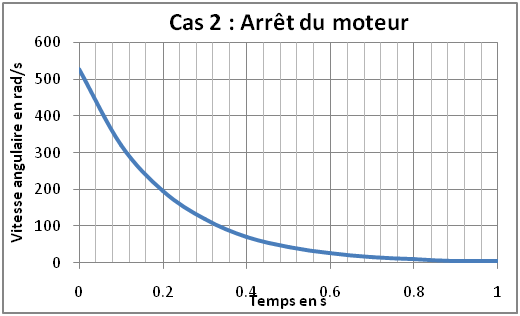
\includegraphics[width=\linewidth]{fig_03}
\end{center}
\end{minipage}
%\subsection{Exponentiation rapide}
%L'exponentiation rapide est un algorithme permettant de calculer $x^n$ en utilisant l'algorithme récursif suivant : 
%$
%\text{puissance}(x,n) =
%\left\{
%\begin{array}{ll}
%x & \text{si }n=1 \\
%\text{puissance}(x^2,n/2) & \text{si } $n$ \text{ est pair} \\
%x\times \text{puissance}(x^2,(n-1)/2) & \text{si } $n$ \text{ est impar pair} \\
%\end{array}
%\right.
%.$
%
%\noindent\begin{minipage}[c]{.45\linewidth}
%\begin{lstlisting}
%def expo_it(x : float, n : int) -> float :
%    res=1
%    while n!=0:
%        if n%2==1:
%            res = res*x
%        x*=x
%        n//=2
%    return res
%\end{lstlisting}
%\end{minipage} \hfill
%\begin{minipage}[c]{.45\linewidth}
%\begin{lstlisting}
%def expo_rec(x : float, n : int) -> float :
%    if n==0:
%        return 1
%    elif n%2==0:
%        return expo_rec(x*x,n//2)
%    else:
%        return x*expo_rec(x*x,n//2)
%\end{lstlisting}
%\end{minipage} 
%



